\subsection{APIC}
To implement the APIC method, we aimed to simulate incompressible fluid behavior with both stability and visual richness. Compared to PIC or FLIP, APIC introduces an affine velocity field per particle to better capture rotational and shear motion, which helps reduce excessive numerical dissipation and jittering effects.

\subsubsection{Algorithm}

The core steps of the APIC method are summarized in Algorithm~\ref{alg:apic}. This method extends the standard PIC approach by introducing an affine velocity matrix for each particle, which allows capturing local rotational and shear motions more accurately.

\begin{algorithm}[h]
\caption{APIC Particle Update Loop}\label{alg:apic}
\begin{algorithmic}[1]

\For{each particle $p$}
\Comment{Particle to Grid (P2G) }
    \For{each neighboring grid node $g$}
        \State Compute weight $w_{pg}$ and offset $\mathbf{d} = x_g - x_p$
        \State Transfer velocity: $v_g \gets v_g + w_{pg} \cdot (v_p + C_p \cdot \mathbf{d})$
        \State Transfer mass: $m_g \gets m_g + w_{pg}$
    \EndFor
\EndFor

\For{each grid node $g$}
\Comment{Grid Operations(Add Forces)}
    \If{$m_g > 0$}
        \State Normalize: $v_g \gets \frac{v_g}{m_g}$
    \EndIf
    \State Apply gravity: $v_g \gets v_g + \Delta t \cdot g$
    \State Enforce boundary conditions on $v_g$
\EndFor

\For{each particle $p$}
\Comment{Grid to Particle (G2P)}
    \State Initialize: $v_p \gets 0$, $C_p \gets 0$
    \For{each neighboring grid node $g$}
        \State Compute weight $w_{pg}$ and offset $\mathbf{d} = x_g - x_p$
        \State Interpolate velocity: $v_p \gets v_p + w_{pg} \cdot v_g$
        \State Update affine matrix: $C_p \gets C_p + w_{pg} \cdot v_g \otimes \mathbf{d}$
    \EndFor
    \State Update position: $x_p \gets x_p + \Delta t \cdot v_p$
\EndFor
\end{algorithmic}
\end{algorithm}

\subsubsection{Intermediate Results and Diagrams}
\begin{figure}[h]
    \centering
    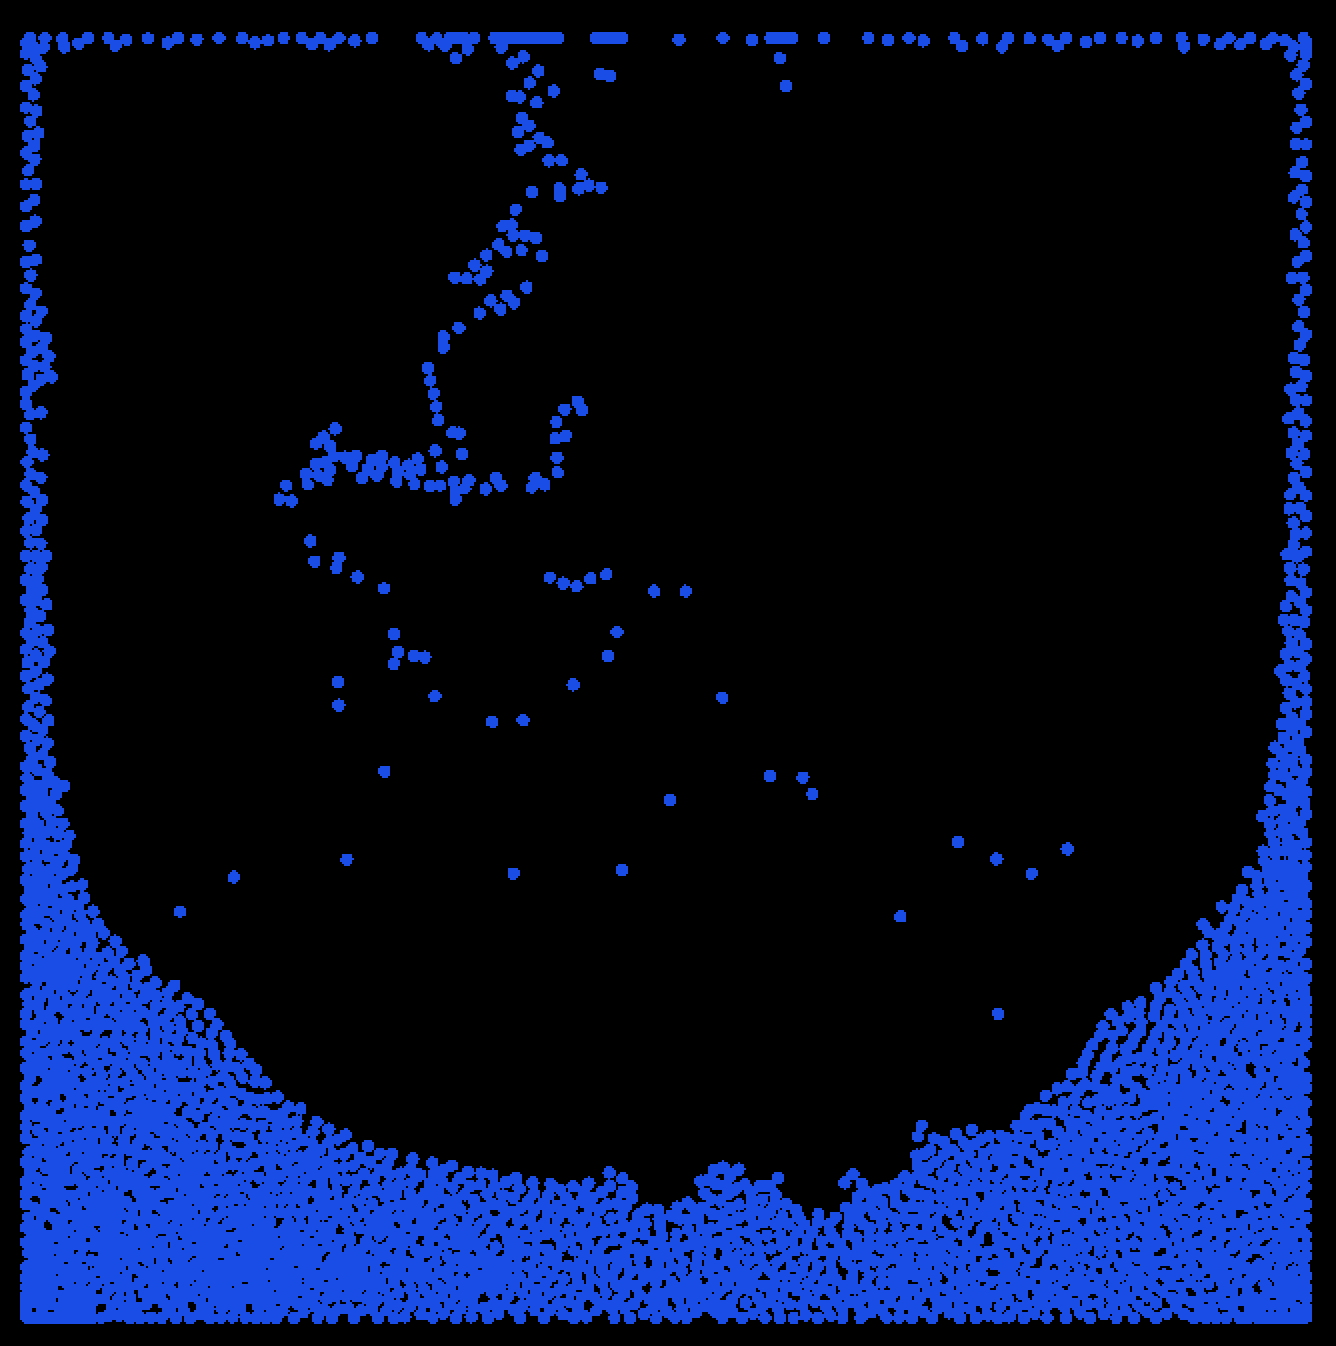
\includegraphics[width=0.25\textwidth]{figures/apic4000.png}
    \caption{Particle distribution in APIC simulation with 4000 particles. }
    \label{fig:apic4000}
\end{figure}

Figure~\ref{fig:apic4000} shows the particle distribution in our APIC simulation using 4000 particles. The APIC method retains coherent motion and prevents clumping or artificial viscosity, which is often observed in simpler schemes like PIC. The particles settle smoothly while preserving rotational features due to the affine velocity transfer.